% 50-minute colloquium talk. Build: latexmk -pdf talk.tex   (figures: python make_figures.py)
\documentclass[aspectratio=169,11pt]{beamer}

% ---- plain style --------------------------------------------------------------
\usetheme{default}
\usefonttheme{professionalfonts}
\setbeamertemplate{navigation symbols}{}
\setbeamertemplate{footline}{\hfill\scriptsize\color{muted}\insertframenumber\hspace{1.2em}\vspace{0.8em}}
\setbeamertemplate{itemize items}{\textbullet}
\setbeamertemplate{frametitle}{\vspace{0.6em}\normalfont\Large\bfseries\insertframetitle}
\setbeamercolor{frametitle}{fg=ink}
\setbeamercolor{title}{fg=ink}
\setbeamercolor{structure}{fg=accent}
\setbeamercolor{normal text}{fg=ink}

\usepackage[T1]{fontenc}
\usepackage{lmodern}
\usepackage{amsmath,amssymb,mathtools}
\usepackage{graphicx}
\usepackage{booktabs}
\usepackage{tikz}
\usetikzlibrary{arrows.meta,positioning,calc,shapes.geometric,decorations.pathreplacing}
\graphicspath{{figures/}}

% colours shared with make_figures.py (extremal.viz)
\definecolor{ink}{HTML}{0B0B0B}
\definecolor{muted}{HTML}{52514E}
\definecolor{accent}{HTML}{EB6834}
\definecolor{blue}{HTML}{3987E5}

% ---- notation -----------------------------------------------------------------
\newcommand{\R}{\mathbb{R}}
\newcommand{\C}{\mathbb{C}}
\newcommand{\Z}{\mathbb{Z}}
\newcommand{\CP}{\mathbb{CP}}
\newcommand{\CPb}{\overline{\mathbb{CP}}{}}
\newcommand{\Lfun}{\mathcal{L}}
\newcommand{\Aext}{A_{\mathrm{ext}}}
\newcommand{\hl}[1]{\textcolor{accent}{#1}}
\newcommand{\aside}[1]{{\small\color{muted}#1}}

% \fig[scale]{file}: make_figures.py draws figures at slide size, so the scale is normally 1
\newcommand{\fig}[2][1]{\begin{center}\includegraphics[scale=#1]{#2}\end{center}}

\tikzset{
  box/.style={draw=ink, rounded corners=3pt, align=center, inner sep=6pt, line width=0.6pt},
  arr/.style={-{Stealth[length=6pt]}, line width=0.8pt, color=muted},
  darr/.style={{Stealth[length=6pt]}-{Stealth[length=6pt]}, line width=0.9pt, color=accent},
}

\title{Extremal metrics on polygons}
\author{Brian Weber}
\date{}

\begin{document}

\begin{frame}[plain]
  \titlepage
\end{frame}

% =================================================================================
% Topic 1: classical mechanics
% =================================================================================

\begin{frame}{Three pictures of mechanics}
  \begin{center}
  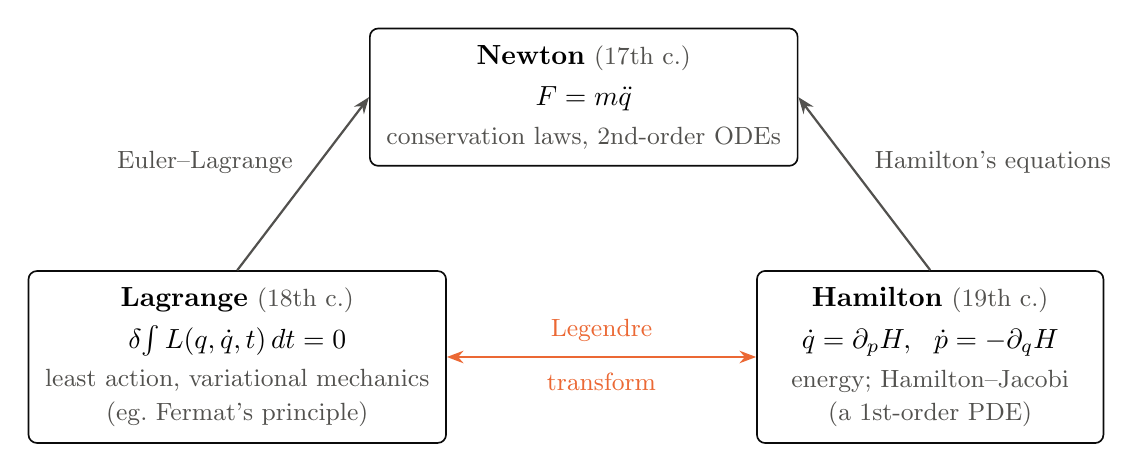
\begin{tikzpicture}[node distance=1cm]
    \node[box, minimum width=4.4cm] (N) at (0, 2.5)
      {\textbf{Newton} \aside{(17th c.)}\\[3pt] $F = m\ddot q$\\[2pt] \aside{conservation laws, 2nd-order ODEs}};
    \node[box, minimum width=4.4cm] (L) at (-4.4, -0.8)
      {\textbf{Lagrange} \aside{(18th c.)}\\[3pt] $\delta\!\int L(q,\dot q,t)\,dt = 0$\\[2pt] \aside{least action, variational mechanics}\\ \aside{(eg.\ Fermat's principle)}};
    \node[box, minimum width=4.4cm] (H) at (4.4, -0.8)
      {\textbf{Hamilton} \aside{(19th c.)}\\[3pt] $\dot q = \partial_p H,\ \ \dot p = -\partial_q H$\\[2pt] \aside{energy; Hamilton--Jacobi}\\ \aside{(a 1st-order PDE)}};
    \draw[arr] (L.north) -- node[above left, font=\small\color{muted}] {Euler--Lagrange} (N.west);
    \draw[arr] (H.north) -- node[above right, font=\small\color{muted}] {Hamilton's equations} (N.east);
    \draw[darr] (L) -- node[above=2pt, font=\small\color{accent}] {Legendre} node[below=2pt, font=\small\color{accent}] {transform} (H);
  \end{tikzpicture}
  \end{center}
\end{frame}

\begin{frame}{The Legendre transform}
  \begin{columns}[c]
    \column{0.48\textwidth}
    \[
      H(q,p,t) \;=\; \dot q_i\,p^i \;-\; L(q,\dot q,t),
      \qquad p^i = \frac{\partial L}{\partial \dot q_i}
    \]
    \vspace{0.5em}
    \begin{itemize}
      \item velocities $\dot q$ \;$\longleftrightarrow$\; momenta $p$
      \item $H(p) = \max_{v}\,\big(p\,v - L(v)\big)$
      \item convex $\leftrightarrow$ convex. Involution: doing it twice gives back $L$
    \end{itemize}
    \column{0.5\textwidth}
    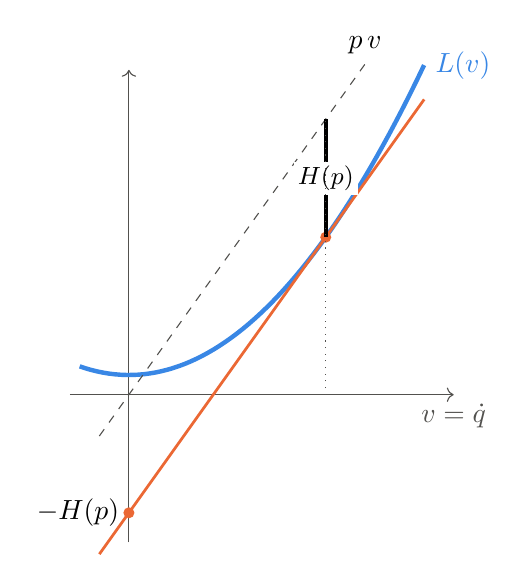
\begin{tikzpicture}[scale=1.25]
      \draw[->, muted] (-0.6,0) -- (3.3,0) node[below] {$v=\dot q$};
      \draw[->, muted] (0,-1.5) -- (0,3.3);
      \draw[blue, line width=1.6pt, domain=-0.5:3.0, samples=60] plot (\x, {0.35*\x*\x + 0.2}) node[right] {$L(v)$};
      % line of slope p = 1.4 through the origin, and the parallel tangent at v = 2
      \draw[muted, dashed] (-0.3,-0.42) -- (2.4,3.36) node[above, black] {$p\,v$};
      \draw[accent, line width=1pt] (-0.3,-1.62) -- (3.0,3.0);
      \fill[accent] (2,1.6) circle (1.6pt);
      \fill[accent] (0,-1.2) circle (1.6pt) node[left, black] {$-H(p)$};
      \draw[line width=1.4pt] (2,1.6) -- (2,2.8);
      \node[fill=white, inner sep=1.5pt, font=\small] at (2,2.2) {$H(p)$};
      \draw[muted, dotted] (2,0) -- (2,2.8);
    \end{tikzpicture}
  \end{columns}
\end{frame}

% =================================================================================
% Topic 2: transition to geometry
% =================================================================================

\begin{frame}{Underneath: symplectic geometry \aside{(20th c.)}}
  A \textbf{symplectic form} on a manifold $M^n$ is a 2-form $\omega$ with
  \[
    d\omega = 0, \qquad \underbrace{\omega\wedge\cdots\wedge\omega}_{n/2} \neq 0 .
  \]
  \begin{itemize}
    \item Classically $\omega = dq_i\wedge dp^i$ \;\aside{(e.g.\ Courant--Hilbert, 1924)}
    \item The \emph{geometry} is $\omega$; the \emph{physics} is a choice of Hamiltonian $H$:
      \[ \omega(X_H,\cdot\,) = dH \quad\leadsto\quad \text{the flow of } X_H \text{ is the action (the kinematic flow)} \]
  \end{itemize}
\end{frame}

\begin{frame}{Phase space}
  \begin{columns}[c]
    \column{0.5\textwidth}
    \begin{itemize}
      \item The cotangent bundle $T^*M$ carries a natural (tautological) symplectic form
        \[ \theta = p^i\,dq_i, \qquad \omega = d\theta. \]
        Invariant form: $v\in TT^*M, (p,q)\in T^*M, \pi:T^*M\rightarrow M$, then
        \[
        \begin{aligned} 
        	&\theta_{(q,p)}(v) = p(\pi_*v), \theta \in T^*T^*M \\
        	&\omega = d\theta \in \bigwedge{}^2T^*M
        \end{aligned}
        \]
      \item A Hamiltonian (or a Lagrangian) creates a Legendre transform.
      This is naturally a linear (on fibers) isomorphism between $T^*M$ and $TM$.
    \end{itemize}
    \column{0.48\textwidth}
    \begin{center}
    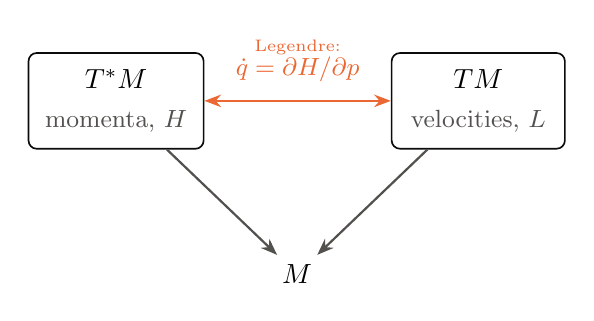
\begin{tikzpicture}
      \node[box, minimum width=2.2cm] (TS) at (0,0) {$T^*M$\\[2pt] \aside{momenta, $H$}};
      \node[box, minimum width=2.2cm] (T) at (4.6,0) {$TM$\\[2pt] \aside{velocities, $L$}};
      \node (M) at (2.3,-2.2) {$M$};
      \draw[darr] (TS) -- node[above=3pt, font=\small] {$\stackrel{\textrm{Legendre:}}{\dot q = \partial H/\partial p}$} (T);
      \draw[arr] (TS) -- (M);
      \draw[arr] (T) -- (M);
    \end{tikzpicture}
    \end{center}
  \end{columns}
\end{frame}

\begin{frame}{A metric is a Hamiltonian}
  \begin{columns}[c]
    \column{0.45\textwidth}
    \begin{itemize}
      \item Kinetic energy $H = \tfrac12\, g^{ij}p_i p_j$.\\
        The metric $g$ is the \emph{polarization} of this quadratic form.
      \item Its Legendre map $T^*M\to TM$ is raising and lowering indices.
      \item Geodesic flow = the motion of a free particle.\\
        Wavefronts solve Hamilton--Jacobi: $|\nabla S|_g = 1$.
    \end{itemize}
    \column{0.53\textwidth}
    \fig{eikonal}
    \vspace{-1.2em}
    \begin{center}\aside{hyperbolic plane: \textcolor{accent}{geodesics} from one point, \textcolor{blue}{wavefronts}}\end{center}
  \end{columns}
\end{frame}

% =================================================================================
% Topic 3: the geometric trifecta
% =================================================================================

\begin{frame}{Three geometries}
  \begin{center}
  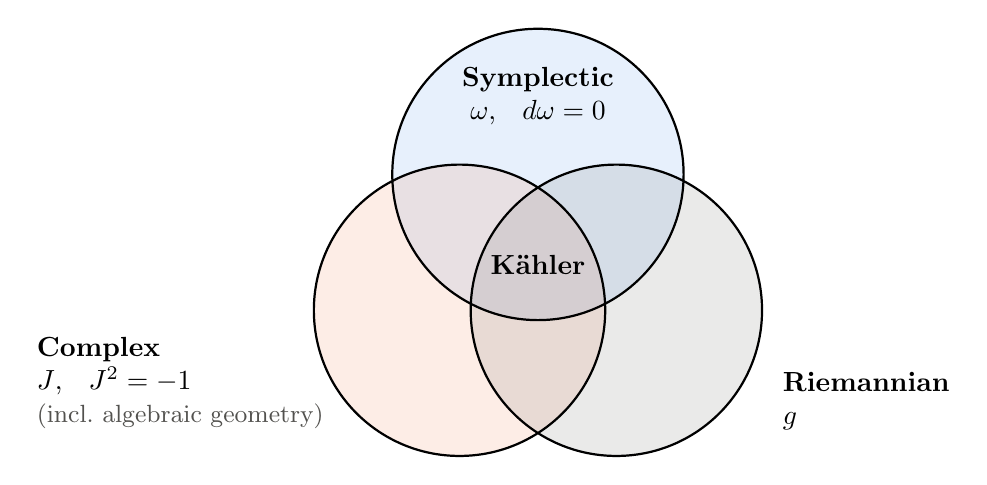
\begin{tikzpicture}
    \def\r{1.85}
    \fill[blue, opacity=0.12] (90:1.15) circle (\r);
    \fill[accent, opacity=0.12] (210:1.15) circle (\r);
    \fill[muted, opacity=0.12] (330:1.15) circle (\r);
    \draw[line width=0.8pt] (90:1.15) circle (\r) (210:1.15) circle (\r) (330:1.15) circle (\r);
    \node[align=center] at (90:2.15) {\textbf{Symplectic}\\ $\omega$, \; $d\omega = 0$};
    \node[align=left, anchor=east] at (210:3.0) {\textbf{Complex}\\ $J$, \; $J^2 = -1$\\ \aside{(incl.\ algebraic geometry)}};
    \node[align=left, anchor=west] at (330:3.45) {\textbf{Riemannian}\\ $g$};
    \node[align=center, font=\bfseries] at (0,0) {Kähler};
  \end{tikzpicture}
  \end{center}
  \vspace{-0.6em}
  \begin{center}
    $g + \omega(J\cdot,\cdot) = 0$
    \qquad\qquad
    \aside{$U(n) = O(2n)\cap Sp(2n,\R)\cap GL(n,\C)$}
  \end{center}
\end{frame}

% =================================================================================
% Topic 4: toric Kähler geometry
% =================================================================================

\begin{frame}{Symmetry}
  \begin{itemize}
    \item Every symmetry gives a conserved quantity: a \textbf{momentum} \aside{(Noether)}.
    \item Phase space of dimension $2n$ with $n$ commuting symmetries:\\
      the motion is \emph{determined}. \aside{(Liouville--Arnold: action--angle variables)}
    \item[]
    \item Kähler manifold of dimension $2n$ with $n$ commuting symmetries (a torus $T^n$):\\
      the \hl{geometry} is determined by the momenta.
    \item[]
    \item The momenta together form the \textbf{moment map} \;$\mu : M^{2n} \to \R^n$.
  \end{itemize}
\end{frame}

\begin{frame}{Moment maps}
  \fig{moment_sphere_cigar}
  \begin{center}
    \aside{rotation about the axis; the moment map is the height. Orbits are circles, which collapse to points at the ends.}
  \end{center}
\end{frame}

\begin{frame}{In dimension 4: a polygon}
  \begin{columns}[c]
    \column{0.5\textwidth}
    \begin{itemize}
      \item $T^2$ acts on $M^4$; \;$\mu : M^4 \to \R^2$.
      \item The image is a convex \textbf{polygon}.
      \item Over each point: the orbit.
      \begin{itemize}
        \item interior: a torus $T^2$
        \item edge: a circle (one circle collapses)
        \item vertex: a point
      \end{itemize}
      \item Coordinates: momenta $x\in P$ and angles $\theta\in T^2$.
    \end{itemize}
    \column{0.48\textwidth}
    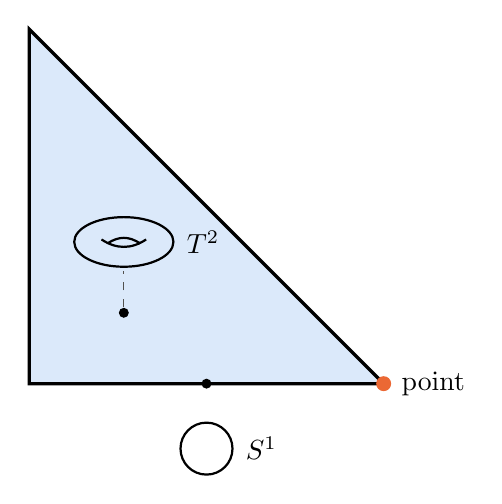
\begin{tikzpicture}[scale=1.5]
      \fill[blue, opacity=0.18] (0,0) -- (3,0) -- (0,3) -- cycle;
      \draw[line width=1.2pt] (0,0) -- (3,0) -- (0,3) -- cycle;
      % torus over an interior point
      \fill (0.8,0.6) circle (1.2pt);
      \begin{scope}[shift={(0.8,1.2)}, scale=0.42]
        \draw[line width=0.8pt] (0,0) ellipse (1 and 0.5);
        \draw[line width=0.8pt] (-0.45,0.05) .. controls (-0.15,-0.15) and (0.15,-0.15) .. (0.45,0.05);
        \draw[line width=0.8pt] (-0.33,-0.03) .. controls (-0.1,0.12) and (0.1,0.12) .. (0.33,-0.03);
      \end{scope}
      \draw[muted, dashed] (0.8,0.65) -- (0.8,0.95);
      \node[right] at (1.25,1.2) {$T^2$};
      % circle over an edge point
      \fill (1.5,0) circle (1.2pt);
      \draw[line width=0.8pt] (1.5,-0.55) circle (0.22);
      \node[right] at (1.75,-0.55) {$S^1$};
      % point over a vertex
      \fill[accent] (3,0) circle (1.8pt) node[right=3pt, black] {point};
    \end{tikzpicture}
  \end{columns}
\end{frame}

% =================================================================================
% Topic 5: Delzant polygons
% =================================================================================

\begin{frame}{Delzant polygons}
  \begin{columns}[c]
    \column{0.55\textwidth}
    \begin{itemize}
      \item \textbf{Delzant} (1988): compact toric symplectic manifolds $\leftrightarrow$ polygons whose edges at each vertex form a basis of $\Z^2$.
      \item $\CP^2$, with $T^2$ acting by $[z_0:z_1:z_2]\mapsto[z_0:e^{i\theta_1}z_1:e^{i\theta_2}z_2]$:
        %\[ \mu = \frac{(|z_1|^2,\,|z_2|^2)}{|z_0|^2+|z_1|^2+|z_2|^2}. \]
        \[ \mu = \left(\frac{|z_1|^2}{|z_0|^2+|z_1|^2+|z_2|^2}, \frac{|z_2|^2}{|z_0|^2+|z_1|^2+|z_2|^2}\right). \]
        The image is a triangle.
    \end{itemize}
    \column{0.42\textwidth}
    \fig{delzant_cp2}
  \end{columns}
\end{frame}

\begin{frame}{Blowing up = cutting off a corner}
  \fig{delzant_blowups}
  \begin{itemize}
    \item One blow-up: the \textbf{Page} Einstein metric is conformal to an extremal Kähler metric on it.
    \item Two blow-ups: so is the \textbf{Chen--LeBrun--Weber} Einstein metric.
  \end{itemize}
\end{frame}

\begin{frame}{The same polygon, another way}
  \fig{delzant_square}
  \begin{center}
    $(\CP^1\times\CP^1)\#\CPb^2 \;\cong\; \CP^2\#2\CPb^2$: \;cutting one corner of the square gives the same pentagon.
  \end{center}
\end{frame}

% =================================================================================
% Topic 6: the symplectic potential
% =================================================================================

\begin{frame}{Geometry on the polygon: the symplectic potential}
  \begin{columns}[c]
    \column{0.5\textwidth}
    \begin{itemize}
      \item One convex function $u$ on $P$ gives the metric
        \[ g = u_{ij}\,dx^i dx^j + u^{ij}\,d\theta_i d\theta_j . \]
      \item Edges $\ell_k(x) = \langle u_k, x\rangle - \lambda_k \ge 0$.
      \item Guillemin's potential
        \[ u_G = \tfrac12 \sum_k \ell_k \log \ell_k \]
        with \hl{log-singularities} at the boundary.
      \item Every toric Kähler metric: $u = u_G + \text{smooth}$ \aside{(Abreu)}.
    \end{itemize}
    \column{0.48\textwidth}
    \fig{guillemin_surface}
    \vspace{-1.5em}
    \begin{center}\aside{$u_G$ as a graph over the $\CP^2$ triangle $P$}\end{center}
  \end{columns}
\end{frame}

% =================================================================================
% Topic 7: Legendre transform and the Kähler potential
% =================================================================================

\begin{frame}{The Legendre transform, again}
  \fig{legendre_toric}
  \[
    \varphi(t) + u(\xi) = \langle t, \xi\rangle, \qquad \xi = \nabla\varphi(t), \qquad t = \nabla u(\xi)
  \]
  \begin{center}\aside{$\varphi$: Kähler potential in log-coordinates $t = \log|z|$ \quad $u$: symplectic potential on the polygon}\end{center}
\end{frame}

\begin{frame}{The fundamental duality}
  \begin{center}
  \renewcommand{\arraystretch}{1.35}
  \begin{tabular}{lcc}
    \toprule
    & \textbf{mechanics} & \textbf{toric Kähler geometry} \\
    \midrule
    one side   & velocities $\dot q$, \; Lagrangian $L$ & complex coordinates $t$, \; Kähler potential $\varphi$ \\
    other side & momenta $p$, \; Hamiltonian $H$          & momenta $\xi\in P$, \; symplectic potential $u$ \\
    relation   & $p = \partial L/\partial\dot q$          & $\xi = \nabla\varphi$ \\
    \midrule
    geometry   & Lagrange \;$\leftrightarrow$\; Hamilton  & \hl{complex} \;$\leftrightarrow$\; \hl{symplectic} \\
    \bottomrule
  \end{tabular}
  \end{center}
\end{frame}

% =================================================================================
% Topic 8: geometrization
% =================================================================================

\begin{frame}{Extremal Kähler metrics}
  \begin{itemize}
    \item Fix the Kähler class. \textbf{Calabi functional}:
      \[ \mathrm{Cal}(g) = \int_M S^2\,d\mu \qquad \text{\aside{($S$ = scalar curvature)}} \]
    \item Its critical points are the \textbf{extremal} metrics: $\nabla S$ is a holomorphic vector field.
    \item Examples:
      \begin{itemize}
        \item constant scalar curvature (cscK)
        \item Kähler--Einstein: $\mathrm{Ric} = \lambda g$
        \item general extremal metrics
      \end{itemize}
    \item[]
    \item Toric: \quad $S = -\tfrac12\,\partial_i\partial_j u^{ij}$ \;\aside{(Abreu)}. \quad Extremal $\iff$ $S$ is an \hl{affine function} on $P$.
  \end{itemize}
\end{frame}

\begin{frame}{Geometrization}
  \textbf{Conjecture.} A Kähler manifold has an essentially unique decomposition into pieces, each of which carries an extremal Kähler metric.
  \aside{(cf.\ Donaldson; Székelyhidi)}
  \fig{q12_pieces}
  \vspace{-0.6em}
  \begin{center}\aside{a polygon with no extremal metric: the best one can do breaks it along a line into $P_1$, $P_2$}\end{center}
\end{frame}

% =================================================================================
% Topic 9: obstructions
% =================================================================================

\begin{frame}{Obstructions: stability}
  \begin{columns}[c]
    \column{0.5\textwidth}
    \begin{itemize}
      \item ``Stability'' comes from geometric invariant theory \aside{(Hilbert, Mumford)}.
      \item To form a quotient by a group, keep only orbits that are \textbf{closed}.
      \item Test with one-parameter subgroups: a sign of a weight.
      \item[]
      \item Here: \hl{instability is an obstruction} to cscK and extremal metrics.
    \end{itemize}
    \column{0.48\textwidth}
    \begin{center}
    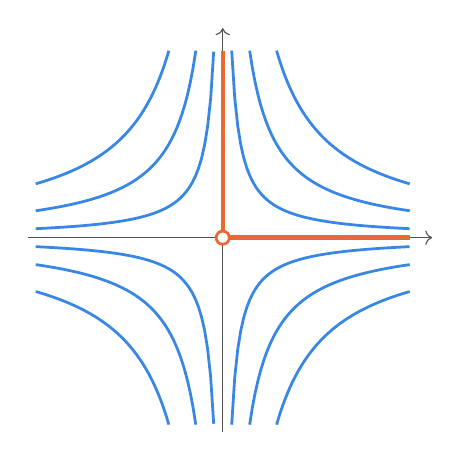
\begin{tikzpicture}[scale=0.95]
      \draw[muted, ->] (-2.6,0) -- (2.8,0);
      \draw[muted, ->] (0,-2.6) -- (0,2.8);
      \foreach \c in {0.3,0.9,1.8} {
        \draw[blue, line width=1pt, domain={\c/2.5}:2.5, samples=60] plot (\x, {\c/\x});
        \draw[blue, line width=1pt, domain={-2.5}:{-\c/2.5}, samples=60] plot (\x, {\c/\x});
        \draw[blue, line width=1pt, domain={\c/2.5}:2.5, samples=60] plot (\x, {-\c/\x});
        \draw[blue, line width=1pt, domain={-2.5}:{-\c/2.5}, samples=60] plot (\x, {-\c/\x});
      }
      \draw[accent, line width=1.6pt] (0.08,0) -- (2.5,0);
      \draw[accent, line width=1.6pt] (0,0.08) -- (0,2.5);
      \draw[accent, line width=1pt, fill=white] (0,0) circle (2.5pt);
    \end{tikzpicture}\\[2pt]
    {\small \textcolor{blue}{hyperbolas: closed orbits (stable)}\\
     \textcolor{accent}{axes: the limit $0$ is not in the orbit}}\\[2pt]
    \aside{$\lambda\cdot(x,y) = (\lambda x, \lambda^{-1}y)$}
    \end{center}
  \end{columns}
\end{frame}

\begin{frame}{The conjecture}
  \begin{center}
  \Large Relatively K-polystable \;$\iff$\; an extremal metric exists
  \end{center}
  \begin{center}\aside{(Yau--Tian--Donaldson; Székelyhidi for extremal metrics)}\end{center}
  \vspace{1em}
  \begin{itemize}
    \item Open in general.
    \item \hl{A theorem for toric surfaces}, i.e.\ for polygons \aside{(Donaldson; Chen--Li--Sheng)}.
    \item[] So polygons are a laboratory where stability can be \emph{computed}.
  \end{itemize}
\end{frame}

% =================================================================================
% Topic 10: the obstruction in the toric case
% =================================================================================

\begin{frame}{The obstruction on a polygon}
  \textbf{Donaldson's linear functional}, for $f$ convex on $P$:
  \[
    \Lfun_A(f) \;=\; \int_{\partial P} f\,d\sigma \;-\; \int_P A\,f\,d\mu
  \]
  \begin{itemize}
    \item $A = \Aext$: the affine function with $\Lfun_A(\text{affine}) = 0$ (computable from $P$).
    \item If $S(u) = A$, integrating by parts gives
      \[ \Lfun_A(f) = \tfrac12\int_P u^{ij} f_{ij}\,d\mu \;\ge\; 0 . \]
    \item \textbf{Stability}: $\Lfun_A(f) > 0$ for every convex, non-affine $f$.
    \item One $f$ with $\Lfun_A(f) < 0$ \hl{proves that no extremal metric exists.}
  \end{itemize}
\end{frame}

\begin{frame}{The nonlinear functional: Donaldson--Mabuchi}
  \[
    \mathcal F(u) \;=\; -\!\int_P \log\det(\mathrm{Hess}\,u)\,d\mu \;+\; 2\,\Lfun_A(u)
  \]
  \begin{center}\aside{Mabuchi's K-energy, written on the polygon (Donaldson)}\end{center}
  \begin{columns}[c]
    \column{0.52\textwidth}
    \begin{itemize}
      \item $\mathcal F$ is \textbf{convex} on symplectic potentials $u = u_G + \text{smooth}$.
      \item $d\mathcal F_u(f) = 2\int_P \big(S(u) - A\big) f\,d\mu$: \\
        critical points $=$ \hl{extremal metrics}.
      \item $\Lfun_A$ is the slope at infinity:
        \[ \mathcal F(u + s f) \;\le\; \mathcal F(u) + 2s\,\Lfun_A(f) . \]
      \item $\Lfun_A(f) < 0$ $\Rightarrow$ $\mathcal F$ is unbounded below \\
        $\Rightarrow$ no minimizer.
    \end{itemize}
    \column{0.46\textwidth}
    \begin{center}
    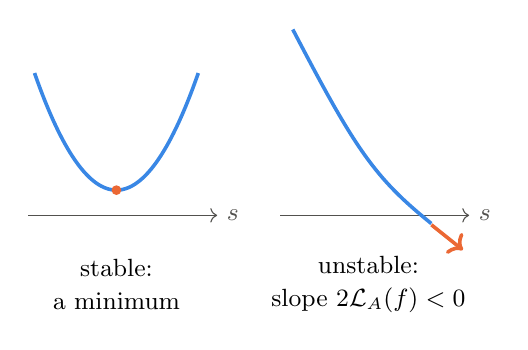
\begin{tikzpicture}[scale=0.8]
      \begin{scope}
        \draw[muted, ->] (-1.4,0) -- (1.6,0) node[right] {\small $s$};
        \draw[blue, line width=1.3pt, domain=-1.3:1.3, samples=60] plot (\x, {1.1*\x*\x + 0.4});
        \fill[accent] (0,0.4) circle (2.2pt);
        \node[align=center] at (0,-1.1) {\small stable:\\ \small a minimum};
      \end{scope}
      \begin{scope}[xshift=4.0cm]
        \draw[muted, ->] (-1.4,0) -- (1.6,0) node[right] {\small $s$};
        \draw[blue, line width=1.3pt, domain=-1.2:1.0, samples=60] plot (\x, {0.4*ln(1+exp(-3*\x)) - 0.75*\x + 0.6});
        \draw[accent, ->, line width=1.3pt] (1.0,-0.15) -- (1.5,-0.55);
        \node[align=center] at (0,-1.1) {\small unstable:\\ \small slope $2\Lfun_A(f) < 0$};
      \end{scope}
    \end{tikzpicture}\\[2pt]
    \aside{$\mathcal F$ along a ray $u + s f$}
    \end{center}
  \end{columns}
\end{frame}

\begin{frame}{Crease functions}
  \begin{columns}[c]
    \column{0.45\textwidth}
    \begin{itemize}
      \item In dimension 2 it suffices to test \textbf{simple creases}
        \[ f = \max(0,\ \ell), \quad \ell \text{ affine} \]
        \aside{(Wang--Zhou)}
      \item One line in the polygon.
      \item Instability = a line with $\Lfun_A(f) < 0$.
    \end{itemize}
    \column{0.53\textwidth}
    \fig{crease_tent}
  \end{columns}
\end{frame}

\begin{frame}{Example: the Wang--Zhou nonagon}
  \begin{columns}[c]
    \column{0.4\textwidth}
    \begin{itemize}
      \item A Delzant polygon: a \emph{smooth} toric surface.
      \item No extremal metric in this class.
      \item Destabilizing line\\ $x + 0.358\,y = 3537.9$
      \item[] \aside{(height parameter $\alpha = 10^4$; found by our code)}
    \end{itemize}
    \column{0.58\textwidth}
    \fig{nonagon}
  \end{columns}
\end{frame}

% =================================================================================
% Topic 11: the code
% =================================================================================

\begin{frame}{The code}
  \begin{center}
  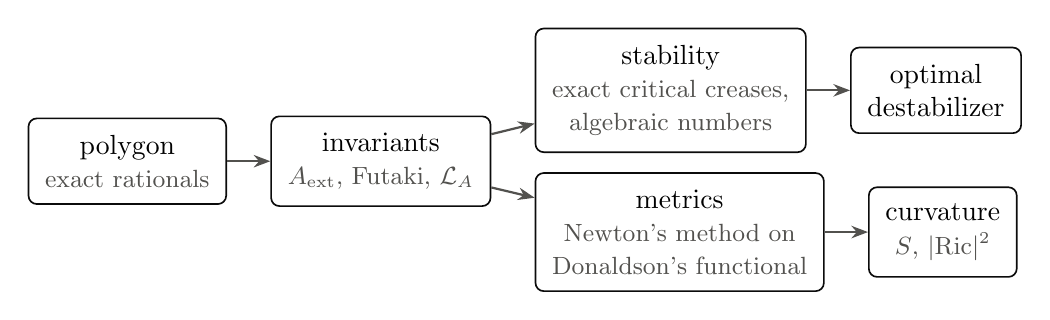
\begin{tikzpicture}[node distance=0.55cm]
    \node[box] (P) {polygon\\ \aside{exact rationals}};
    \node[box, right=of P] (I) {invariants\\ \aside{$\Aext$, Futaki, $\Lfun_A$}};
    \node[box, right=of I, yshift=0.9cm] (S) {stability\\ \aside{exact critical creases,}\\ \aside{algebraic numbers}};
    \node[box, right=of I, yshift=-0.9cm] (M) {metrics\\ \aside{Newton's method on}\\ \aside{Donaldson's functional}};
    \node[box, right=of S] (D) {optimal\\destabilizer};
    \node[box, right=of M] (C) {curvature\\ \aside{$S$, $|\mathrm{Ric}|^2$}};
    \draw[arr] (P) -- (I);
    \draw[arr] (I) -- (S);
    \draw[arr] (I) -- (M);
    \draw[arr] (S) -- (D);
    \draw[arr] (M) -- (C);
  \end{tikzpicture}
  \end{center}
  \vspace{0.5em}
  \begin{itemize}
    \item Approximate extremal metrics: minimize
      the Donaldson--Mabuchi functional $\mathcal F$ over $u = u_G + \text{polynomial}$.
    \item Python; \texttt{github.com/lapisetanima/toric-kahlers}
  \end{itemize}
\end{frame}

\begin{frame}{Orbifolds: easier to destabilize}
  \fig{labels_q4_q12}
  \begin{itemize}
    \item A \textbf{label} $m$ on an edge: cone angle $2\pi/m$ along that divisor.
    \item Same quadrilateral, labels $(1,4,4,4)$ and $(1,12,12,12)$: one has an extremal metric, the other does not.
  \end{itemize}
\end{frame}

\begin{frame}{When there is no metric, the approximation goes haywire}
  \fig{solver_haywire}
  \begin{columns}[t]
    \column{0.42\textwidth}
    \small
    \begin{tabular}{rcc}
      \toprule
      degree & $Q_4$ & $Q_{12}$ \\
      \midrule
      10 & 0.21  & $1.0\cdot 10^3$ \\
      14 & 0.064 & $10$ \\
      18 & 0.022 & $4.6\cdot 10^3$ \\
      \bottomrule
    \end{tabular}\\[2pt]
    \aside{$\|S - A\|_{L^2}$ (area-normalized). For $Q_{12}$ it is at least $0.064$.}
    \column{0.55\textwidth}
    \begin{itemize}
      \item $Q_4$: the approximations converge.
      \item $Q_{12}$: they cannot. A \emph{global} polynomial can't break along the line.
      \item The right answer is piecewise: $S \to A - f^*$.
    \end{itemize}
  \end{columns}
\end{frame}

\begin{frame}{Exact answers}
  \begin{columns}[c]
    \column{0.5\textwidth}
    \fig{q12_optimal_crease}
    \column{0.48\textwidth}
    \textbf{Optimal destabilizer} of $Q_{12}$:
    \begin{itemize}
      \item line $x + m\,y = s$, \;$m = 1.65238288\ldots$
      \item $m$ is a root of an integer polynomial of degree 18
      \item $\|f^*\| = 0.16417411137442506876\ldots$
      \item[] \aside{a lower bound for $\|S - \Aext\|$ over all toric metrics}
    \end{itemize}
  \end{columns}
\end{frame}

\begin{frame}{A threshold}
  \fig{threshold}
  \vspace{-0.5em}
  \[
    \lambda^* = 4.31756909532834813881399236429256191048568\ldots
  \]
  \begin{center}\aside{exact critical creases; confirmed independently by Apostolov--Calderbank--Gauduchon's criterion for quadrilaterals}\end{center}
\end{frame}

% =================================================================================
% Topic 12: AI
% =================================================================================

\begin{frame}{A testbed for AI}
  \begin{itemize}
    \item Answers are \textbf{exactly checkable}: a destabilizing line is a certificate.
    \item Problems are cheap to generate, with tunable difficulty.
    \item Disguised: no mention of Kähler geometry; the model gets a Python tool.
  \end{itemize}
  \vspace{0.8em}
  \begin{center}
  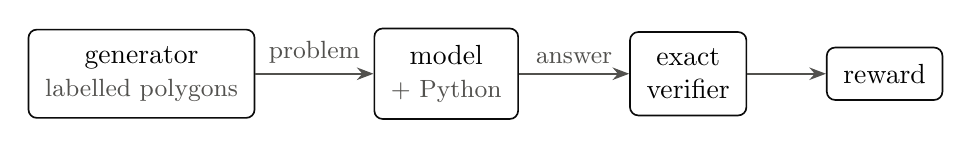
\begin{tikzpicture}[node distance=0.6cm]
    \node[box] (G) {generator\\ \aside{labelled polygons}};
    \node[box, right=1.5cm of G] (Mo) {model\\ \aside{+ Python}};
    \node[box, right=1.4cm of Mo] (V) {exact\\verifier};
    \node[box, right=1cm of V] (R) {reward};
    \draw[arr] (G) -- node[above, font=\small\color{muted}] {problem} (Mo);
    \draw[arr] (Mo) -- node[above, font=\small\color{muted}] {answer} (V);
    \draw[arr] (V) -- (R);
  \end{tikzpicture}
  \end{center}
\end{frame}

\begin{frame}{Tasks \aside{(work in progress)}}
  \begin{itemize}
    \item \textbf{Classify}: stable or unstable?
    \item \textbf{Certify}: produce a line with $\Lfun_A < 0$. \aside{Checked exactly.}
    \item \textbf{Optimize}: the optimal line, to as many digits as possible. \aside{Reward $\sim$ digits correct.}
  \end{itemize}
  \vspace{1em}
  \begin{itemize}
    \item Quadrilaterals have a closed-form theory \aside{(Apostolov--Calderbank--Gauduchon)}: too easy to look up.
    \item Pentagons and beyond: no closed form. \hl{This is where models must discover something.}
  \end{itemize}
\end{frame}

\begin{frame}[plain]
  \begin{center}
    \Large Thank you
  \end{center}
\end{frame}

\end{document}
